\documentclass[unicode,11pt,a4paper,oneside,numbers=endperiod,openany]{scrartcl}
\usepackage{listings}
\usepackage{amsmath}

\usepackage{pgfplots}
\pgfplotsset{compat=newest}

\renewcommand{\thesubsection}{\arabic{subsection}}

\usepackage{ifthen}
\usepackage[utf8]{inputenc}
\usepackage{graphics}
\usepackage{graphicx}
\usepackage{hyperref}

\pagestyle{plain}
\voffset -5mm
\oddsidemargin  0mm
\evensidemargin -11mm
\marginparwidth 2cm
\marginparsep 0pt
\topmargin 0mm
\headheight 0pt
\headsep 0pt
\topskip 0pt        
\textheight 255mm
\textwidth 165mm

\newcommand{\duedate} {}
\newcommand{\setduedate}[1]{%
\renewcommand\duedate {\textbf{Due date:}~ #1}}
\newcommand\isassignment {false}
\newcommand{\setassignment}{\renewcommand\isassignment {true}}
\newcommand{\ifassignment}[1]{\ifthenelse{\boolean{\isassignment}}{#1}{}}
\newcommand{\ifnotassignment}[1]{\ifthenelse{\boolean{\isassignment}}{}{#1}}

\newcommand{\assignmentpolicy}{
\begin{table}[h]
\begin{center}
\scalebox{0.8} {%
\begin{tabular}{|p{0.02cm}p{16cm}|}
\hline
&\\
\multicolumn{2}{|c|}{\Large\textbf{Numerical Computing 2023 ---  Submission Instructions}}\\
\multicolumn{2}{|c|}{\large\textbf{(Please, notice that following instructions are mandatory: }}\\
\multicolumn{2}{|c|}{\large\textbf{submissions that don't comply with, won't be considered)}}\\
&\\
\textbullet & Assignments must be submitted to \href{https://www.icorsi.ch/course/view.php?id=14666}{iCorsi} (i.e. in electronic format).\\
\textbullet & Provide both executable package and sources (e.g. C/C++ files, MATLAB). 
If you are using libraries, please add them in the file. Sources must be organized in directories called:\\
\multicolumn{2}{|c|}{\textit{Project\_number\_lastname\_firstname}}\\
& and  the  file must be called:\\
\multicolumn{2}{|c|}{\textit{project\_number\_lastname\_firstname.zip}}\\
\multicolumn{2}{|c|}{\textit{project\_number\_lastname\_firstname.pdf}}\\
\textbullet &  The TAs will grade your project by reviewing your project write-up, and looking at the implementation you attempted, and benchmarking your code's performance.\\

\textbullet & You are allowed to discuss all questions with anyone you like; however: (i) your submission must list anyone you discussed problems with and (ii) you must write up your submission independently.\\
\hline
\end{tabular}
}
\end{center}
\end{table}
}
\newcommand{\punkte}[1]{\hspace{1ex}\emph{\mdseries\hfill(#1~\ifcase#1{Points}\or{Points}\else{Points}\fi)}}


\newcommand\serieheader[6]{
\thispagestyle{empty}%
\begin{flushleft}

\includegraphics[width=0.45\textwidth]{CI_logo}
\end{flushleft}
  \noindent%
  {\large\ignorespaces{\textbf{#1}}\hspace{\fill}\ignorespaces{ \textbf{#2}}}\\ \\%
  {\large\ignorespaces #3 \hspace{\fill}\ignorespaces #4}\\
  \noindent%
  \bigskip
  \hrule\par\bigskip\noindent%
  \bigskip {\ignorespaces {\Large{\textbf{#5}}}
  \hspace{\fill}\ignorespaces \large \ifthenelse{\boolean{\isassignment}}{\duedate}{#6}}
  \hrule\par\bigskip\noindent%  \linebreak
 }

\makeatletter
\def\enumerateMod{\ifnum \@enumdepth >3 \@toodeep\else
      \advance\@enumdepth \@ne
      \edef\@enumctr{enum\romannumeral\the\@enumdepth}\list
      {\csname label\@enumctr\endcsname}{\usecounter
        {\@enumctr}%%%? the following differs from "enumerate"
	\topsep0pt%
	\partopsep0pt%
	\itemsep0pt%
	\def\makelabel##1{\hss\llap{##1}}}\fi}
\let\endenumerateMod =\endlist
\makeatother




\usepackage{textcomp}







\begin{document}


\setassignment
\setduedate{Wednesday, December 20, 2023, 11:59 PM}

\serieheader{Numerical Computing}{2023}{Student: Hun Rim}{Discussed with: Georgy Batyrev}{Solution for Project 5}{}
\newline

\assignmentpolicy


The purpose of this project is to implement the Simplex Method to find the solution of linear programs, involving both the minimisation and the maximisation of the objective function.

\section{Graphical Solution of Linear Programming Problems [20 points]}
Please consider the following two problems:
\begin{enumerate}
	\item[(1)] \begin{equation*}
		\begin{aligned}
		& \text{min}  &  z=4x&+y\\
		& \text{ s.t.} &  x+2y &\leq 40 \\
		& &   x+y &\geq 30\\
		& &   2x+3y &\geq 72 \\
		& &  x,\,y &\geq0 \\
		\end{aligned}
		\end{equation*}
	\item[(2)] A tailor plans to sell two types of trousers, with production costs of 25 CHF and 40 CHF, respectively. The former type can be sold for 85 CHF, while the latter for 110 CHF. The tailor estimates a total monthly demand of 265 trousers. Find the number of units of each type of trousers that should be produced in order to maximise the net profit of the tailor, if we assume that the he cannot spend more than 7000 CHF in raw materials.
\end{enumerate}
Start by writing problem (2) as a linear programming problem. Then complete the following tasks:
\begin{itemize}
	\item Solve the system of inequalities.
	\item Plot the feasible region identified by the constraints.
	\item Find the optimal solution and the value of the objective function in that point.
\end{itemize}

\vspace{20px}

\begin{enumerate}
 \item[Sol (1.1)] The optimal solution to the equation (1) is as the following. According to the line segment between the inequality functions, it is easy to identify that the optimal minimum value of ${z = 106}$ at the point ${P=(24,8)}$. There are 2 other vertices, one at (36, 0) which results in ${z}$ to be 144 and another at (40, 0) which results in ${z}$ to be 160. Hence, optimal minimum value of ${x = 24}$ and ${y = 8}$. Graphed result of the min(z) linear programming problem is as following, where the optimal point is highlighted with a \textbf{red circle}: \\
\begin{figure}[h!]
    \begin{minipage}[c]{1\linewidth}
        \centering
        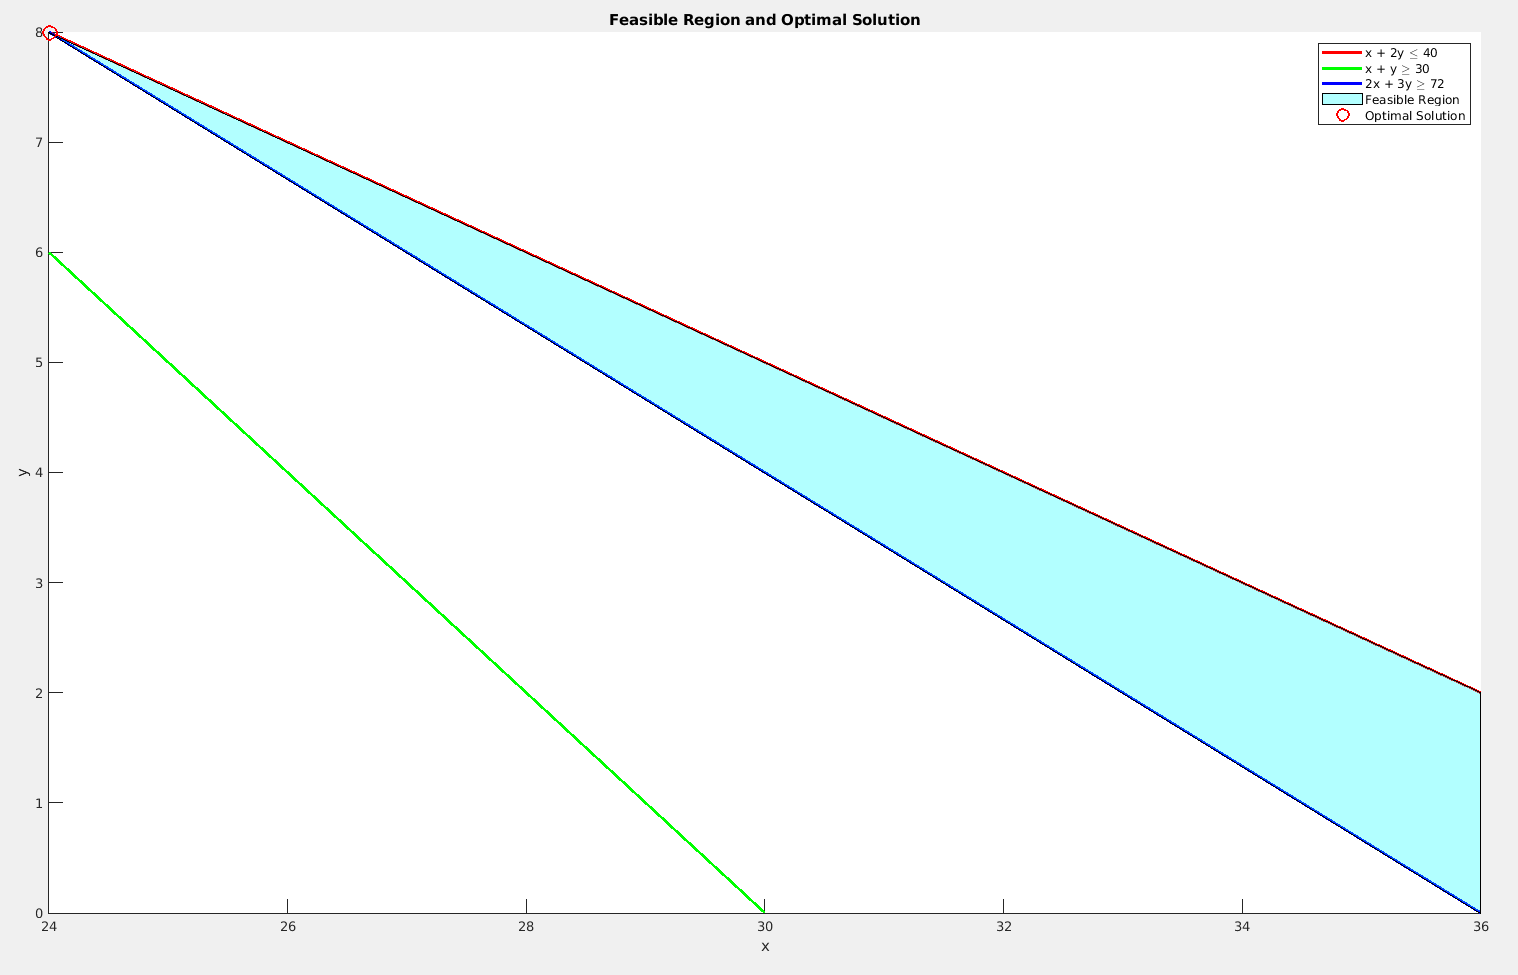
\includegraphics[width=0.9\linewidth]{./figure1.png}
    \end{minipage}
    \caption{Plotted optimal region of linear programming problem (1)}
\end{figure}

Please refer to ${ex1a.m}$ script to see the code used to calculate the optimal minimum and find the feasible area. \\

\item[Sol (1.2)] First, the trouser production problem has to be converted to a linear programming problem using the information given in the text. Under the assumption ${z = saleProfit}$, \\ ${x = aQuantity(60CHF/profitPerPiece)}$, ${y = bQuantity(70CHF/profitPerPiece)}$, we can write the equation linear programming problem as the following: \\

\begin{equation*}
		\begin{aligned}
		& \text{max}  &  z=60x&+70y\\
		& \text{ s.t.} &  25x+40y &\leq 7000 \\
		& &   x+y &\leq 265\\
		& &  x,\,y &\geq0 \\
		\end{aligned}
		\end{equation*}
\end{enumerate}

Demand is constrained by 265 so sum of ${x}$ and ${y}$ is limited by it, and the maximum production cost (7000CHF) limits the value of ${x}$ (25CHF for production) and ${y}$ (40CHF for production). Naturally, ${x, y}$ has to be greater than 0, although, not given. \\

\begin{figure}[h!]
    \begin{minipage}[c]{1\linewidth}
        \centering
        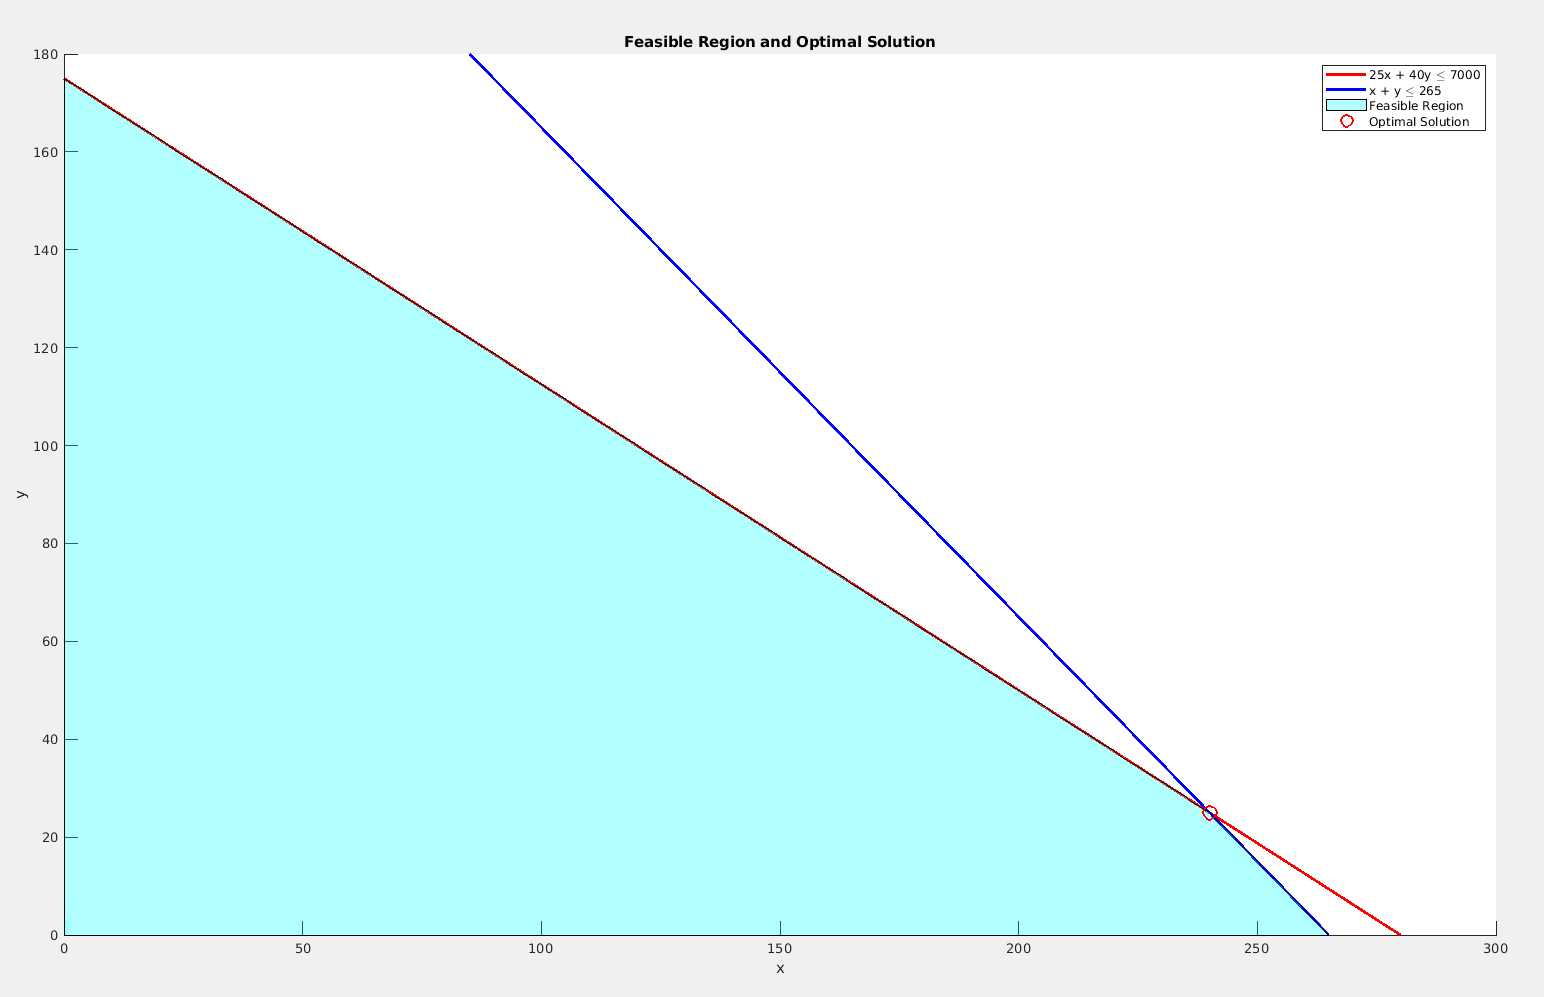
\includegraphics[width=0.9\linewidth]{./figure2.png}
    \end{minipage}
    \caption{Plotted optimal feasible region of trouser production problem}
\end{figure}

As explained before, the optimal feasible region is highlighted in light-blue color and the optimal value of ${z}$ through vertices of the polytope. Found maximum profit (including the production cost) is ${max(z) = 16150 CHF}$ by producing 240 ${trouserA}$ and 25 ${trouserB}$. (${optimal(x)=240}$, ${optimal(y)=25}$) There were other vertexes at (265, 0) which gave profit of ${15900CHF}$ and at (0, 175) which gave ${12250CHF}$ but the maximum was at (240, 25). \\

\begin{lstlisting}[language=Matlab]
    c = [-60; -70];

    A = [25, 40; 1, 1];
    b = [7000; 265];

    lowerBounds = [0; 0];

    options = optimoptions('linprog', 'Display','off');
    [x, fval, exitflag] = linprog(c, A, b, [], [], lowerBounds, [], options);
    
    ... Print the optimal solution and Plot the Graph ...
\end{lstlisting}

\vspace{20px}

One thing to note is that the values of ${c}$ are multiplied by ${-1}$ unlike the solution of the first problem because the first problem was looking for a minimum, but here the solution sought for is the maximum. The vertice of polytope (intersection of line segment) and the optimal solution of the linear programming problem was calculated using ${linprog}$ Matlab function, similar to the solution of linear programming problem (1). Please refer to the ${ex1b.m}$ script to view the implementation for the whole solution. 


\section{Implementation of the Simplex Method [30 points]}

In this first part of the assignment, you are required to complete 2 functions which are part of a dummy implementation of the simplex method. Specifically you have to complete the TODOs in:
\begin{itemize}
	\item \emph{standardise.m}, which writes a maximisation or minimisation input problem in standard form;
	\item \emph{simplexSolve.m}, which solves a maximisation or minimisation problem using the simplex method.
\end{itemize}
You are given also some already-implemented functions to help you in your task: \emph{simplex.m} is a wrapper which calls all the functions necessary to find a solution to the linear program; \emph{auxiliary.m} solves the auxiliary problem to find a feasible starting basic solution of the linear program; \emph{printSol.m} is a function which prints the optimal solution found by the simplex algorithm. Finally, \emph{testSimplex.m} presents a series of 6 problems to check if your implementation is correct, before moving to the next part of the assignment. Additional details to aid you in your implementation can be found in the comments inside the code. \\

\begin{enumerate}
 \item[Sol(2):] All the implementations are given in the ${standardise.m}$, ${simplexSolve.m}$, and ${simplex.m}$ scripts in the ${Project5\_Files\_and\_Data}$ folder. All the tests from the ${testSimplex.m}$ script passes. \textit{Please refer to the scripts to see the implementation.}
\end{enumerate}


\section{Applications to Real-Life Example: Cargo Aircraft [25 points]}

In this second part of the assignment, you are required to use the simplex method implementation to solve a real-life problem taken from economics (constrained profit maximisation).

A cargo aircraft has 4 compartments (indicated simply as $S_1,\dots,S_4$) used to store the goods to be transported. Details about the weight capacity and storage capacity of the different compartments can be inferred from the data reported in the following table: 

\begin{center}
 \begin{tabular}{||c | c | c ||} 
 \hline
 Compartment & Weight Capacity ($t$) & Storage Capacity ($m^3$) \\ [0.5ex] 
 \hline\hline
 $S_1$ & 18 & 11930\\ 
 \hline
 $S_2$ & 32 & 22552\\
 \hline
 $S_3$ & 25 & 11209\\
 \hline
 $S_4$ & 17 & 5870\\
 \hline
\end{tabular}
\end{center}

The following four cargos are available for shipment during the next flight:

\begin{center}
 \begin{tabular}{|| c | c | c | c ||} 
 \hline
 Cargo & Weight ($t$) & Volume ($m^3/t$) & Profit ($\text{CHF}/t$) \\ [0.5ex] 
 \hline\hline
 $C_1$ & 16  & 320 & 135 \\ 
 \hline
 $C_2$ & 32  & 510 & 200 \\
 \hline
 $C_3$ & 40 & 630 & 410 \\
 \hline
 $C_4$ & 28 & 125 & 520 \\
 \hline
\end{tabular}
\end{center}

Any proportion of the four cargos can be accepted, and the profit obtained for each cargo is increased by $10\%$ if it is put in $S_2$, by $20\%$ if it is put in $S_3$ and by $30\%$ if it is put in $S_4$, due to the better storage conditions. The objective of this problem is to determine which amount of the different cargos will be transported and how to allocate it among the different compartments, while maximising the profit of the owner of the cargo plane. Specifically you have to:
\begin{enumerate}
	\item Formulate the problem above as a linear program: what is the objective function? What are the constraints? Write down all equations, with comments explaining what you are doing.
	\item Create a script \emph{exercise2.m} which uses the simplex method implemented in the previous exercise to solve the problem. What is the optimal solution? Visualise it graphically and briefly comment the results obtained (are you surprised of this outcome on the basis of your data?).
\end{enumerate}

\vspace{20px}

\begin{enumerate}
 \item[Sol(3.1)]Formulation of the problem into a linear program: \\
 
 To simplify the problem, there are 4 cargos and 4 compartments with all the necessary information. To calculate which configuration can maximize the profit, the problem can be converted to an objective function.
 
 \begin{center}
\begin{equation*}
\begin{aligned}
\text{max z}= (135x_{11} + 200x_{12} + 410x_{13} + 520x_{14}) +\\
 1.1(135x_{21} + 200x_{22} + 410x_{23} + 520x_{24}) + \\
 1.2(135x_{31} + 200x_{32} + 410x_{33} + 520x_{34}) + \\
 1.3(135x_{41} + 200x_{42} + 410x_{43} + 520x_{44}) 
\end{aligned}
\end{equation*}

\end{center}

Where ${x_{ij}}$ represents the Cargo ${j}$ stored in Compartment ${i}$. \\

\textbf{Constraints}:
\begin{enumerate}
 \item Non-negative value constraints:
 \begin{equation*}
  x_{ij} >= 0, \text{ where } 0 \leq i,j \leq 4
 \end{equation*}
 \item Compartment Weight Constraints(Sum of cargo weight in compartment should not exceed the compartment weight limit):
 \begin{equation*}
  \begin{aligned}
   x_{11} + x_{12} + x_{13} + x_{14} \leq 18 \\
   x_{21} + x_{22} + x_{23} + x_{24} \leq 32 \\
   x_{31} + x_{32} + x_{33} + x_{34} \leq 25 \\
   x_{41} + x_{42} + x_{43} + x_{44} \leq 17 \\
  \end{aligned}
 \end{equation*}
 \item Compartment Volume Constraints (Sum of cargo volume in compartment should not exceed the compartment volume limit):
 \begin{equation*}
  \begin{aligned}
   320x_{11} + 510x_{12} + 630x_{13} + 125x_{14} \leq 11930 \\
   320x_{21} + 510x_{22} + 630x_{23} + 125x_{24} \leq 22552 \\
   320x_{31} + 510x_{32} + 630x_{33} + 125x_{34} \leq 11209 \\
   320x_{41} + 510x_{42} + 630x_{43} + 125x_{44} \leq 5870 \\
  \end{aligned}
 \end{equation*}
 
  \item Cargo Weight Constraints (Sum of weight beloning to Cargo ${j}$ in all Compartments should be equivalent or less than total weight of Cargo ${j}$):
 \begin{equation*}
  \begin{aligned}
   x_{11} + x_{21} + x_{31} + x_{41} \leq 16 \\
   x_{12} + x_{22} + x_{32} + x_{42} \leq 32 \\
   x_{13} + x_{23} + x_{33} + x_{43} \leq 40 \\
   x_{14} + x_{24} + x_{34} + x_{44} \leq 28 \\
  \end{aligned}
 \end{equation*}

\end{enumerate}

\item[Sol(3.2)] According to the found linear program, the solution has been implemented in the ${exercise2.m}$ script. Result of optimal solution has been calculated through the implemented ${simplex()}$ function from the ${simplex.m}$. The result is as the following: \\

\begin{center}
\begin{tabular}{l|l|l|l|l|r}
 & ${S_1}$ & ${S_2}$ & ${S_3}$ & ${S_4}$ & Total Cargo \\
 \hline
 ${C_1}$ & 0 & 0 & 0 & 0 & 0 \\
  \hline
 ${C_2}$ & 18 & 6 & 0 & 0 & 24 \\
  \hline
 ${C_3}$ & 0 & 26 & 14 & 0 & 40 \\
  \hline
 ${C_4}$ & 0 & 0 & 11 & 17 & 28 \\
  \hline
 Compartment Cargo & 18 & 32 & 25 & 17 & \\
\end{tabular}
\end{center}

According to the optimal solution found through the ${simplex}$ method, the maximum profit is ${41890 CHF}$.

In conclusion, none of the cargo 1 has been moved, 24 out of 32 cargos were moved out of cargo 2. Rest of cargo 3 and 4 were transported. Due to it, all the compartments were completely filled. As a result, maximum total profit estimated was ${41,890 CHF}$. As expected, the cargo with higher profit was placed in the compartment with higher profit increase. Because the compartment capacity was visibly lower than amount of cargo present, as a result, cargo 1 and 2 which had low profit was completely left out or at least some of it was left out as expected. Although, maximum total profit calculated from the information was certainly lower than what was expected from the first look.  
\end{enumerate}

\section{Cycling and Degeneracy [10 points]}

Consider now the following simple problem:
\begin{alignat*}{2}
	&\text{max}\;\, && z = 3x_1+4x_2,\\
	&\text{s.t.} && 4x_1+3x_2\leq 12\\
	& && 4x_1+x_2\leq 8\\
	& && 4x_1+2x_2\leq 8\\
	& && x_1, x_2 \geq 0.
\end{alignat*}

\begin{enumerate}
	\item Create a script \emph{exercise3.m} which uses the simplex method implemented above to solve this problem. Do you achieve convergence within the maximum number of iterations (given by the maximum number of possible basic solutions)? Do you notice any strange behaviour? (\emph{hint:} check, e.g., the indices of the entering and departing variables)
	\item Look at the number of constraints and at the number of unknowns: what can you notice about the underlying system of equations? Represent them graphically and try to use this information to explain the behaviour of your solver in the previous point. 
\end{enumerate}

\begin{enumerate}
 \item[Sol(4.1)] The equation can be re-structured as the following to be solved with simplex method:
 \begin{equation*}
  c=\begin{bmatrix}
     3 \\ 4 \\ 0 \\ 0 \\ 0\\
    \end{bmatrix},
    A=\begin{bmatrix}
       4 & 3 & 1 & 0 & 0 \\
       4 & 1 & 0 & 1 & 0 \\
       4 & 2 & 0 & 0 & 1 \\
      \end{bmatrix},
    h=\begin{bmatrix}
       12 \\ 8 \\ 8 \\
      \end{bmatrix}
 \end{equation*}

 Running the ${exercise3.m}$ results in displaying an error message. Which means the convergence wasn't achieved within the maximum number of set iterations which was calculated to be 56. Also from printing the index\_in and index\_out, it seems it is cycling between the 2 and 4, hence, it is not converging I am assuming.\\
 
 \newpage
 
 The value of x\_B is as the following in the final iteration in the given limit.
 
 \begin{center}
  \begin{equation*}
   x\_B=\begin{bmatrix}
         4 \\ 2 \\ 0 \\
        \end{bmatrix}
  \end{equation*}
 \end{center}
 
 The value of x\_B was the same for many iterations. Which makes sense as a basic feasible solution containing 0 is a degenerate solution indicating a potential source of error in the constraints.\\
 
 \item[Sol(4.2)] Visualization of the linear programming problem:
 \begin{center}
 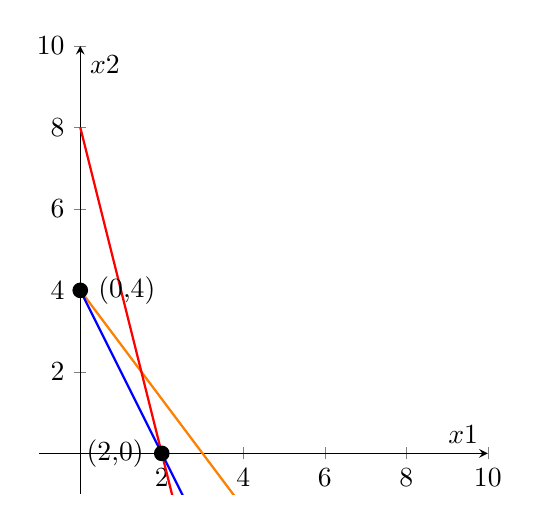
\begin{tikzpicture}
\begin{axis}[
	xmin=-1, xmax=10,
	ymin=-1, ymax=10,
	axis lines=center,
	axis equal image,
	xlabel=$x1$,
	ylabel=$x2$,
]

\addplot[domain=0:6, samples=100, orange, thick] {4 - 4/3*x};
\addplot[domain=0:6, samples=100, red, thick] {8 - 4*x};
\addplot[domain=0:6, samples=100, blue, thick] {4 - 2*x};
\node[label={0:{(0,4)}},circle,fill,inner sep=2pt] at (axis cs:0,4) {};
\node[label={180:{(2,0)}},circle,fill,inner sep=2pt] at (axis cs:2,0) {};
\end{axis}
\end{tikzpicture}
\end{center}
Now the problem is graphed, we can clearly see that the constraints fail to form a feasible region due to the linearly dependent constraints. This would be a possible reason for the failure of the simplex method causing the algorithm to swap between the same set of basic feasible solutions without converging towards a final solution. In other words, there was a 'cycle' formed due to the degenerate solution. We need to remove dependent or redundant constraints to avoid this problem.
\end{enumerate}


\section{Quality of the Code \& Report [15 points]}

Each project sums up to 100 points, out of which 15 points are dedicated to the general quality of your written report and of the code submitted. Your report should be a coherent document. If there are theoretical questions, explain and justify your answers. If you made a particular choice in your implementation that might be out of the ordinary, please explain it in the report. The code you submit should be self-contained and executable. It should include the set-up for all the results that you obtained and listed in your report. Furthermore, it should be readable and include comments explaining the more complicated steps.


\end{document}
